\documentclass[11pt]{report}
\usepackage[utf8]{inputenc}
\usepackage[french]{babel}
\usepackage[T1]{fontenc}
\usepackage{geometry}
\usepackage{graphicx}
\usepackage{svg}
\usepackage{amsmath}
\usepackage{float}
\usepackage{hyperref}
\usepackage{tikz}
\usepackage{booktabs}
\usepackage{cite}
\usepackage[skip=10pt, indent=20pt]{parskip}

\geometry{
a4paper,
left=1in,
top=1in,
right=1in,
bottom=1in,
}

\newcommand\Chapter[2]{
  \chapter[#1: {\itshape#2}]{#1\\[2ex]\large\itshape#2}
}

\title{Rapport du projet intégré: groupe 2}
\author{Joey Brynckman, Andrea Dal Molin, Thibault Havet, Florent Raeymaeckers,  \\ Arnaud Rase, William Tea, Lionel Thys \& Alexandre Villance}
\date{Q2 2022-2023}

\begin{document}

\maketitle

\tableofcontents

\chapter*{Abstract}

Ce rapport est un descriptif du projet sur lequel nous avons travaillé en tant qu'équipe d'étudiant de la Haute école de la Province de Liège. Nous devions mettre en place un système de paiement sur base d'un énoncé donné durant le mois de Mars 2023. Le but est d'avoir une plateforme qui peut être accédée par un utilisateur qui souhaite effectuer un paiement en ligne vers un marchand.

Notre solution à ce problème regroupe de l'authentification, de l'exploration de données, de la sécurisation de données et du déploiement de serveurs. Nous allons développer ces points ci-dessous.

\chapter{Introduction de l'équipe}

Notre équipe est composée de 8 personnes:

\paragraph{Joey Brynckman}
\paragraph{Andrea Dal Molin}
\paragraph{Thibault Havet}
\paragraph{Flo Raeymaeckers} (DevOps \& Responsable Équipe)

Je me suis occupée de l'infrastructure logicielle du déploiement de la solution. Plus précisément, j'ai mis en place un cluster de serveurs afin que l'ensemble des services que l'on voulait déployer sur le serveur puisse profiter d'un load balancing et d'une virtualisation par container afin d'avoir une scalabilité horizontale des services en fonction de la demande.

De plus, j'ai géré l'équipe. J'ai travaillé sur la mise en commun des ressources (réunions, outils de suivi de projet...), de ce rapport, et enfin de la présentation que vous allez pouvoir assister. Je vais passer en revue dans ce document les différentes difficultés par lesquelles je suis passée et les éventuelles solutions que j'ai apporté.

\paragraph{Arnaud Rase}
\paragraph{William Tea}
\paragraph{Lionel Thys}
\paragraph{Alexandre Villance}

\chapter{Étude et mise en théorie de l'infrastructure}

Dans ce chapitre, nous allons passer en revue l'étude que nous avons effectué sur l'énoncé du projet transmit pas nos professeurs. Le projet part d'un énoncé basé sur une version "simplifiée" de 3D secure, ou du moins plus ou moins cousine: nous avons un marchand qui souhaite pouvoir proposer à ses clients la vente de ses services/bien en ligne. Afin que le consommateur puisse payer, le marchand a besoin d'une plateforme de paiement en ligne. Notre rôle est d'implémenter cette plateforme de payement au niveau de la banque du consommateur, qui va alors se synchroniser avec la banque du marchand pour valider la transaction.

\section{Schéma de l'infrastructure}

\part{Implémentation des services}


\Chapter{Déploiement de l'infrastructure}{Arnaud Rase \& Flo Raeymaeckers}

\section{Virtualisation des services}

\begin{figure}[H]
    \centering
    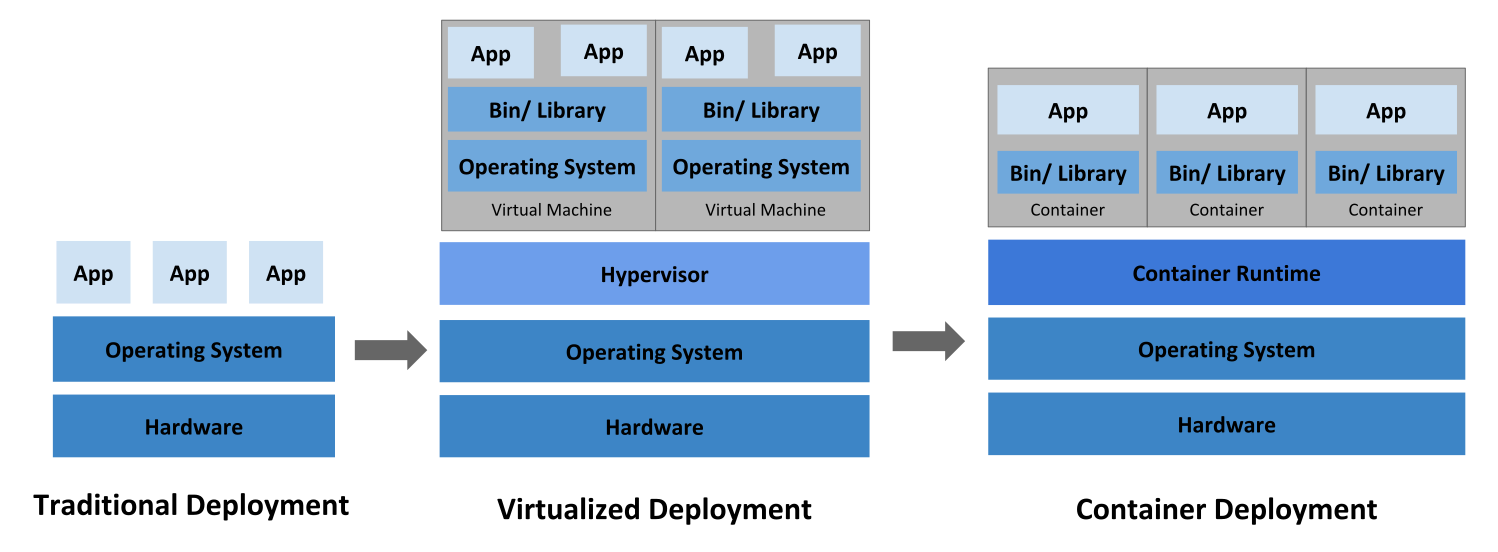
\includegraphics[width=\textwidth]{./img/container_evolution.png}
    \caption{Évolution du déploiement d'applications \cite{shavidissa2019}}
    \label{fig:container_evolution}
\end{figure}

\Chapter{Mise en place de la topologie réseau}{Arnaud Rase}

\Chapter{Configuration d'un service d'authentification centralisé}{Lionel Thys}

\Chapter{Création d'une application marchande PoC}{Joey Brynckman}

\Chapter{Mise en place d'une cellule d'analyse de données}{Thibault Havet}

\Chapter{Module d'authentification par carte d'identité et gestion de points de fidélité par smartcard}{Andrea Dal Molin}

\Chapter{Testing et assurance qualité des produits}{Alexandre Villance \& Flo Raeymaeckers}

\Chapter{Gestion de l'équipe}{Flo Raeymaeckers}

\chapter{Améliorations du projet}

\section{Niveau de l'exécution du projet}

\section{Niveau de la gestion d'équipe}

\bibliographystyle{plain}
\bibliography{ref}

\end{document}
